\documentclass[titlepage]{article}
\usepackage{a4wide}
\usepackage{graphicx}
\usepackage{csvsimple}

\begin{document}

\title{MultiAgent Systems \\ An Efficient and Robust Disaster Recovery}
\author{Anis Jonischkeit}

\maketitle

\section{Introduction}
  This report will briefly explain why the hybrid agent architecture was chosen (and is suitable) for this task. It will then go into depth describing the implementation, pros and cons of the design, and an analysis of the results obtained.

\section{The Hybrid Agent Architecture}
  For the first project in this course, we were given the task of designing a reactive agent architecture. A reactive architecture generally takes some sensory input and produces some action. Although this solved the described task, it wasn't perfect. There was no co-ordination between agents and a lack of a symbolic representation. The purely reactive rescue units were still a major part of the 2nd project, however this time there were a few other agents in the world. A base agent was introduced which rescue agents could use to send basic messages to. This base agent was also a reactive agent since it works by receiving an event and reacting to it. 
  \\ \\
  The ambulances, which were the biggest change in the second assignment were based on a hybrid agent architecture. This hybrid architecture consisted of both the reactive architecture and a Deliberative (pro-active) architecture. This pro-active architecture gave a huge advantage to the ambulances as it allowed them to perform complex tasks in the dynamic disaster environment. 
  \\ \\
  The ambulances followed the BDI (beliefs, desires, intentions) deliberative model. The beliefs of an agent consist of what the agent believes to be true of the world. These beliefs (in my program) consist of the civilians that have been located by the rescue agents. The Intentions consist of the agent's current plan for achieving these goals. The desires were not explicitly represented in the program however each ambulances desires were always to rescue as many agents as quickly as possible. BDI is what made it possible to hold auctions on who should go where and make sure that if an ambulance breaks down that victims wouldn't become neglected.
  \\ \\
  The ambulances also had a reactive part very similar to the rescue agents, which would make the ambulances move to the base to drop of civilians when the ambulance got full. Another reactive task that ambulances would do is picking up victims.
  \\ \\
  As you can see, both the reactive and pro-active architectures served different goals and both brought a lot of value to the ambulances and how well they could cope with the disaster situation. Neither a purely reactive or purely pro-active architecture would have been able to achieve the task as well as the combination of the architectures did.

\section{Problem 1 and 2}
  \subsection{Solution Sketches}
    To solve problem 1, instead of making all agents go to `collect' their first belief, the agents should instead go to their closest belief. Whenever a new civilian is found, the ambulances also clear their intentions and re-assign new intentions to themselves according to their new beliefs.
    \\ \\
    To solve problem 2, I made sure that when an ambulance saves a civilian, that ambulance will broadcast a message to the other ambulances, letting them know that the civilian has been saved. Receiving this message will prompt the ambulances to remove the collect belief of the specific civilian. They will also all clear their intentions and re-assign new intentions to themselves according to their new beliefs. Although it is not always necessary to clear the intentions for all of the ambulances, it doesn't harm to remove everyone's intentions and just makes it a bit simpler to implement. The ambulance will re-assign its intentions before executing them anyway.
    
  \subsection{Observations}
    The solutions implemented still make some agents follow each other since a civilian may be the closest for multiple agents, however it is a lot better than the original especially if there are many civilians. Some might argue that when an ambulance starts going to a civilian, the other ambulances should remove the civilian from their beliefs (so that they won't go there). This would however lead to civilians becoming stranded. If something was to go wrong with ambulances breaking down, the civilian would be stranded and no ambulance would know.

  \subsection{Results and Analysis}
    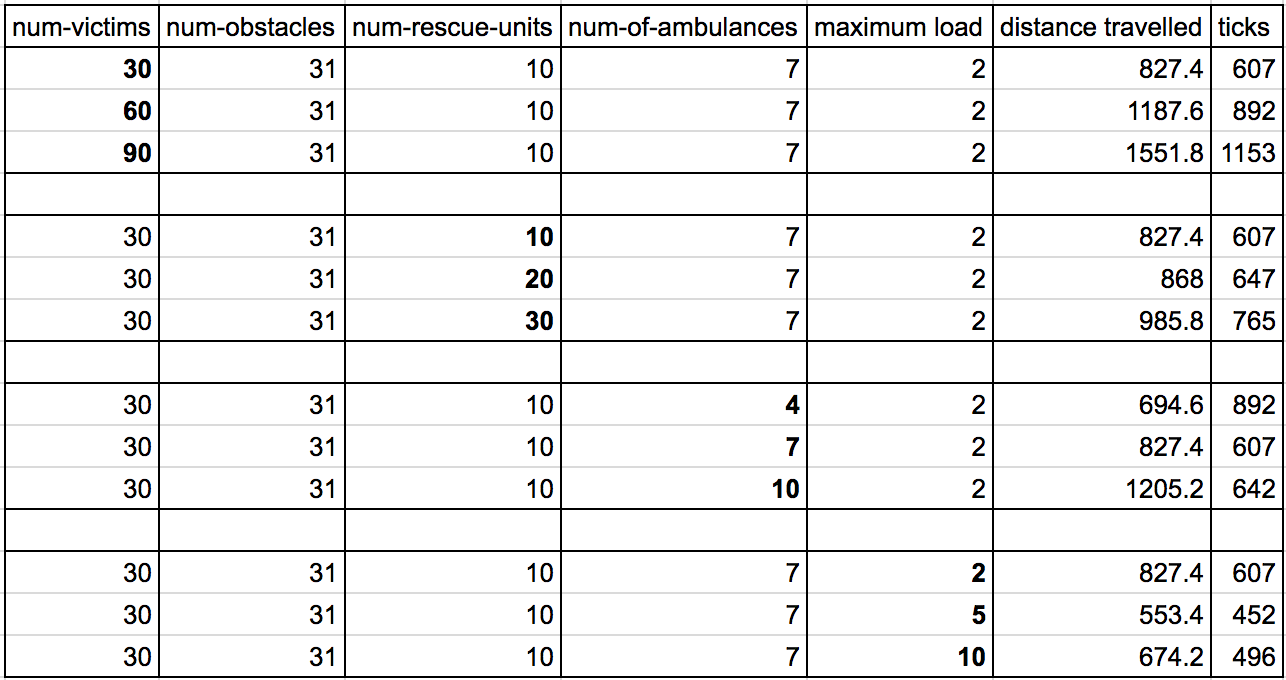
\includegraphics[width=\textwidth,height=\textheight,keepaspectratio]{1table.png}
    \\
    Above is a table of tests that I have conducted. all tests used seed 44. Modifications to the program setup are bolded.
    \\
    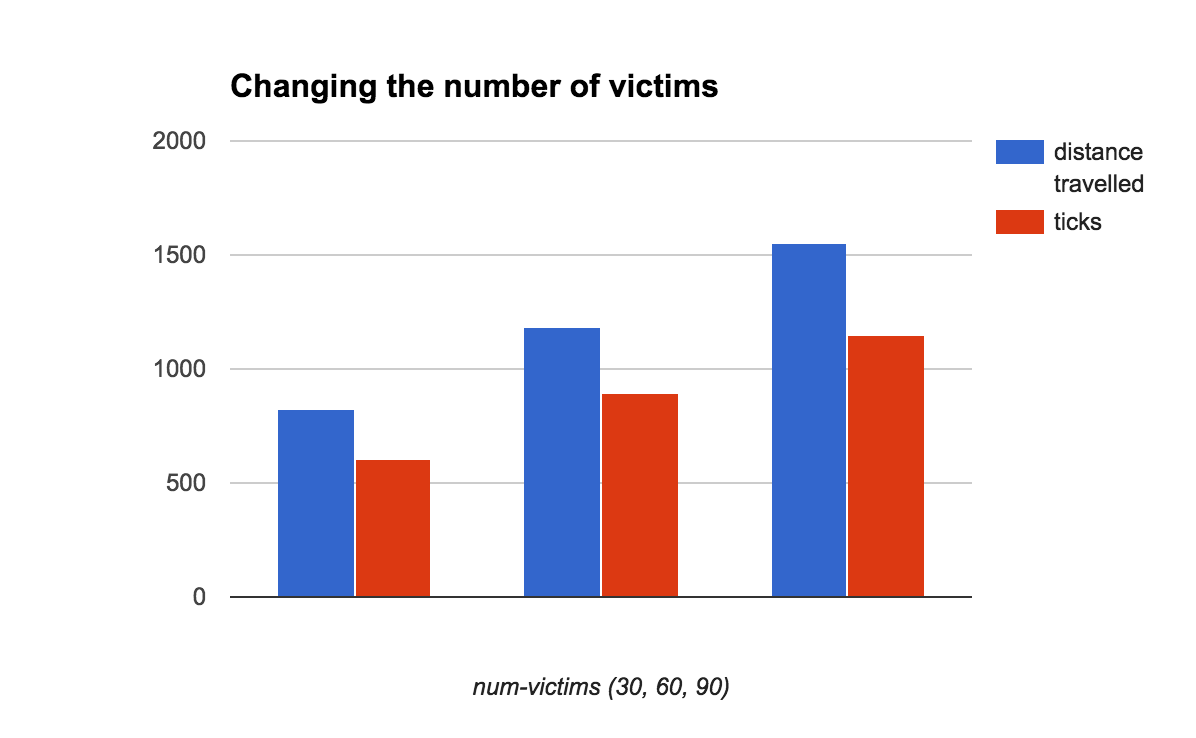
\includegraphics[width=\textwidth,height=\textheight,keepaspectratio]{1victims.png}
    \\
    As expected, increasing the number of victims, increases both fuel consumption and time taken to complete the rescue.
    \\
    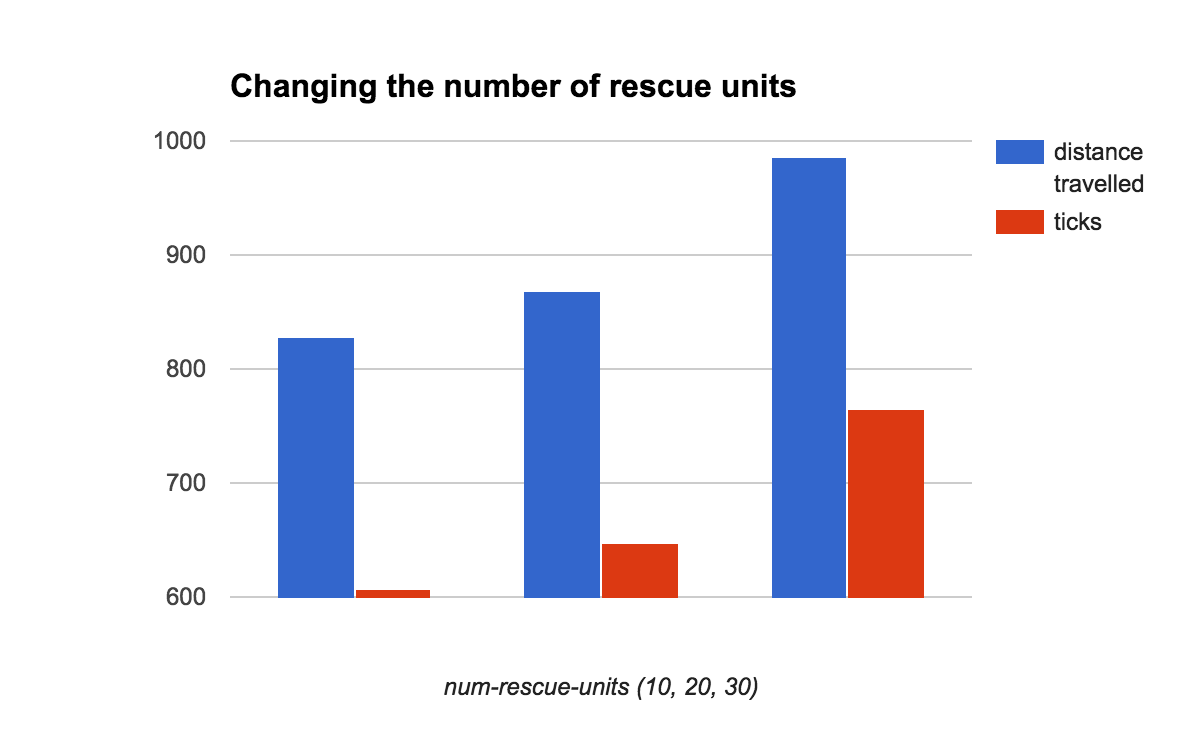
\includegraphics[width=\textwidth,height=\textheight,keepaspectratio]{1rescueunits.png}
    \\
    Surprisingly enough, increasing the number of rescue units actually increases both the time taken and the fuel usage. This is because of the fact that having too many rescue agents stops the rescue agents from being able to move around properly, slowing down the search process.
    \\
    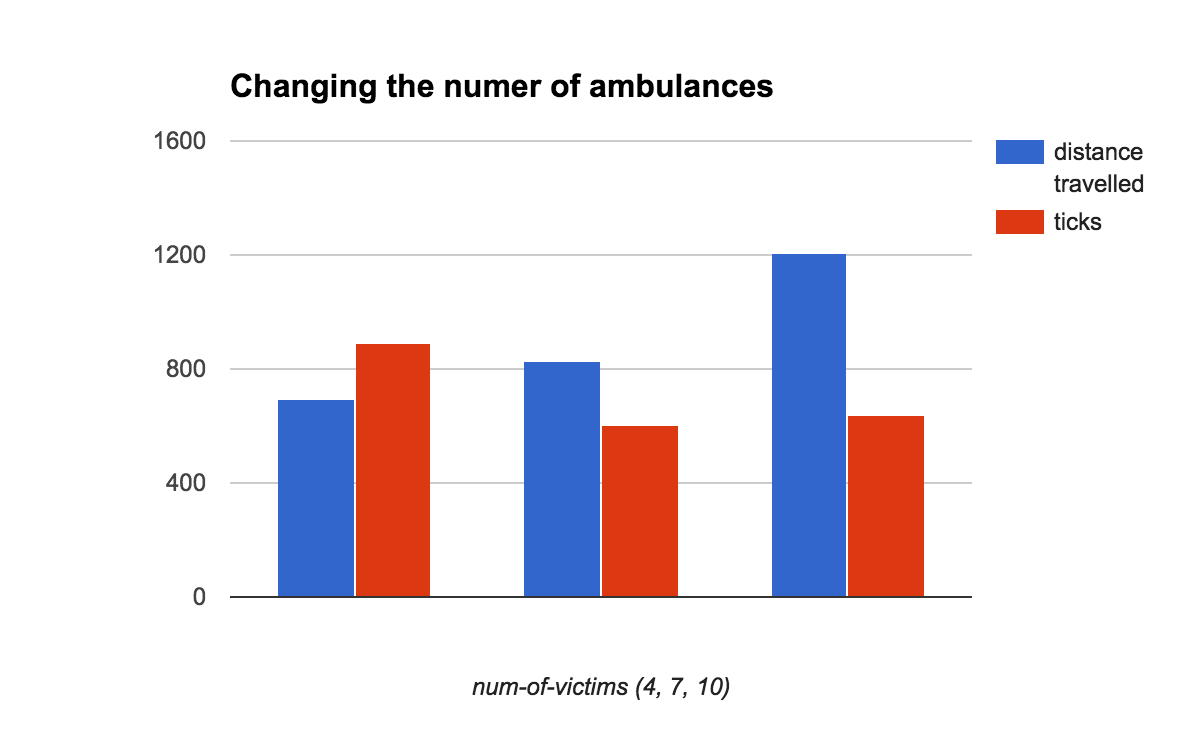
\includegraphics[width=\textwidth,height=\textheight,keepaspectratio]{1ambs.png}
    \\
    Increasing the number of ambulances from 4 to 7 definitely makes a difference, however there is no real difference between 7 and 10. This is due to the fact that with so many ambulances, they wouldn't split up enough to make a noticeable difference.
    \\
    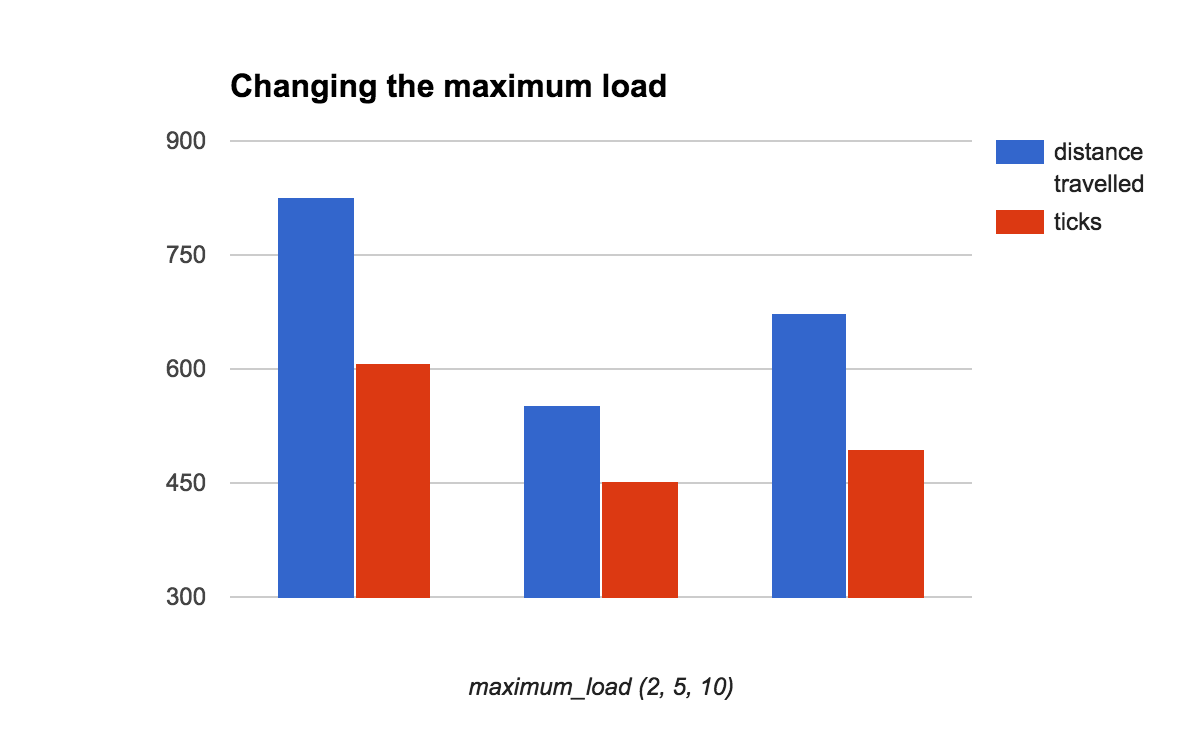
\includegraphics[width=\textwidth,height=\textheight,keepaspectratio]{1load.png}
    \\
    Increasing the load from 2 to 5 civilians decreases the time taken for the rescue mission. This is because the ambulances don't have to go back to the base all the time. When the load is however increased to 10, the time taken actually goes up. This is just because of the fact that with this seed, by chance the ambulances actually pick up a few civilians while leaving the base and re-basing gets them a bit more spread out.
  
  \subsection{Lessons Learned}
    I believe that the biggest problem to this approach is that multiple ambulances do still go to the same civilian if that civilian is closest to them. This problem will be addressed while approaching problem 3.

\section{Problem 3}
  \subsection{Solution Sketches}
    For problem 3 there were two main objectives that I was looking out for. I wanted to make the system as robust as possible and I wanted to make the system as efficient as it could be.
    \\ \\
    In order to make the system as robust as possible I needed to make sure that there would never be a single point of failure. The first thing that needed to be changed from the Problem 2 implementation was the communication with the base station. There cannot be any communication with the base station since there is only one which causes a really serious single point of failure (if the base station goes down, the system goes down). To get rid of this communication, I made the rescue agents broadcast the `collect' message directly to the ambulances, rather than going through the base-station.
    \\ \\
    The next issue I wanted to tackle was the fact that when each agent would go to its closest found civilian, multiple agents could end up going to save the same civilian. To make sure that only the closest ambulance goes to pick up a specific civilian, I decided to implement a bidding system. Whenever a civilian is found, each ambulance bids on the civilian that is currently closest to them. The bid consists of the co-ordinate of the civilian and the distance that the agent is away from the civilian.
    \\ \\
    On the next step, each agent works out whether they would win the bid. Each auction only consists of one round so one round after a bid was started there is sure to have been a winner. If an ambulance doesn't win the bid it makes sure to add all locations that have already been bidded on to a blacklist of co-ordinates that are already or are going to be occupied. This blacklist only lasts for the step. 
    \\ \\
    When an agent wins an auction, we need to make sure that other agents don't go to the same location. Removing the belief is one way of doing this however this isn't very robust. If the ambulance that is picking up the victim breaks down, then the victim will be stranded. Also if the ambulance wants to pick up someone else instead, no-one else will know that the specific civilian is free to be picked up. In order to prevent these issues, each ambulance that is picking up a civilian must broadcast that it is picking up the specific civilian. This broadcast will be saved by the other ambulances for two ticks and if the message isn't received again within those two ticks, other ambulances can tell that the victim actually does still need to be picked up. This allows for ambulances that are already picking up a civilian to take part in bids, and another ambulance can take over that ambulances original task if the bid is won. Ambulances will however only bid while they are picking someone up if the new civilian is closer to them than the one they are currently going after.
    \\
    \\
    There was a line in the code telling the ambulances to wait for 30 ticks before starting to do anything. This line wastes 30 ticks in which ambulances could be saving people so I removed this waiting time.
    \\
    \\
    One last improvement that I made is that when an ambulance has no beliefs that aren't being fulfilled by another ambulances, the ambulance will move randomly, just like the rescue agents. There is no point in having ambulances sit in the same spot waiting for civilians to be found, when they can look too. If a civilian is found by a rescue unit, the ambulance will stop moving randomly and pick up the civilian, but otherwise, if the ambulance has nothing to do, it will move randomly. Something interesting I have noticed is that the ambulances move a lot quicker when they are moving randomly than when they are using the gps direction.
  
  \subsection{Observations}
    Watching the ambulance pick up the civilians, you can really see that there is a lot of organisation going on. The ambulances do not follow each other to go to the same civilian and they become very good at all picking up different civilians at the same time. One thing I added to test the robustness of the system is a chance of ambulance breakdown. This is a slider that you can slide to increase or decrease the probability of ambulances breaking down. It is very interesting to watch when an ambulance breaks down as when this happens, if there aren't other civilians to collect, other agents will immediately take over from where the other ambulance died.
    \\
    \\
    I had a problem in the beginning where ambulances without intentions would come back to the base and then stop, blocking the base. As soon as I implemented the `move-randomly when there are no intentions that can be made' feature, this problem fixed itself since nobody would wait at the base.
    \\
    \\
    Since ambulances are faster when they move randomly, you can see a jump in speed for just one tick when they get to the base. This happens since they bid, but haven't won a bid yet. So for 1 tick they have no intentions and will move randomly.
    \\
    \\
    Since the ambulances all go for their closest civilian, what ends up happening is that the ambulances will going to the base and the slowly going outwards from the base collect civilian. This is quite interesting to watch since in the end you just see a ring of green civilians on the outside of the map.

  \subsection{Results and Analysis}
    Below is a table showing the results of the same tests as for the Problem 1/2 solution:
    \\
    \\
    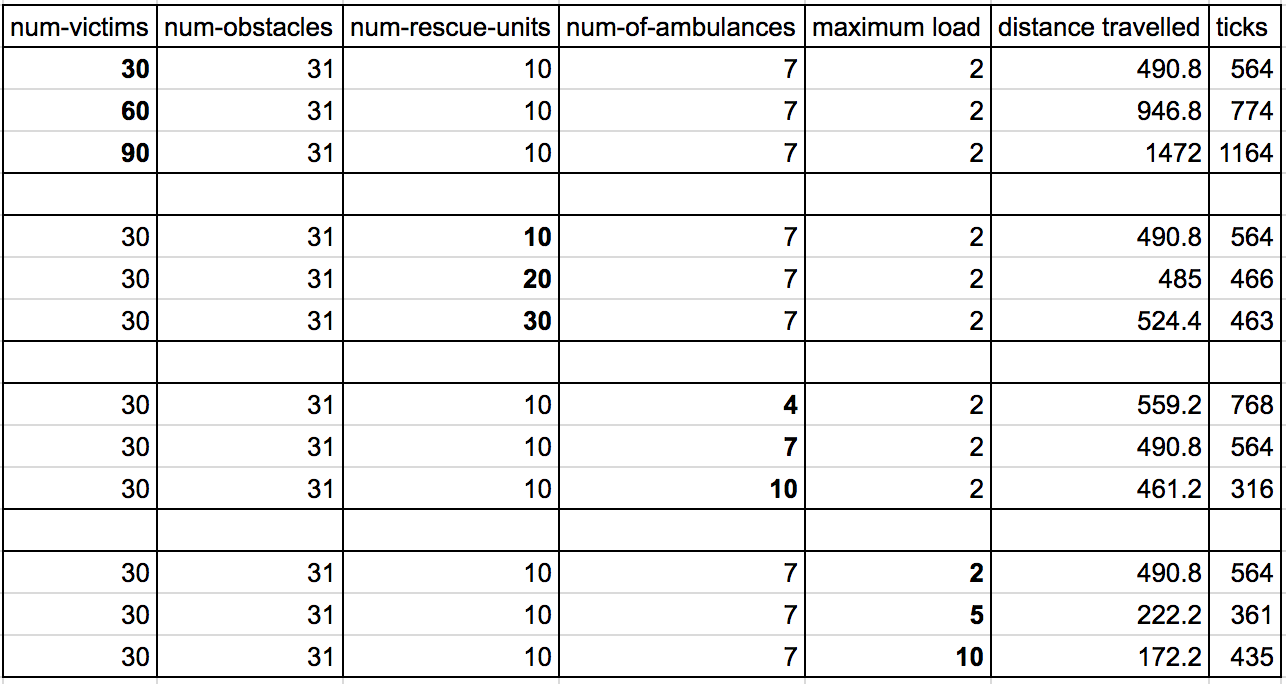
\includegraphics[width=\textwidth,height=\textheight,keepaspectratio]{2table.png}
    \\
    \\
    You can already see that the average time taken is a lot lower than on the previous implementation.
    \\
    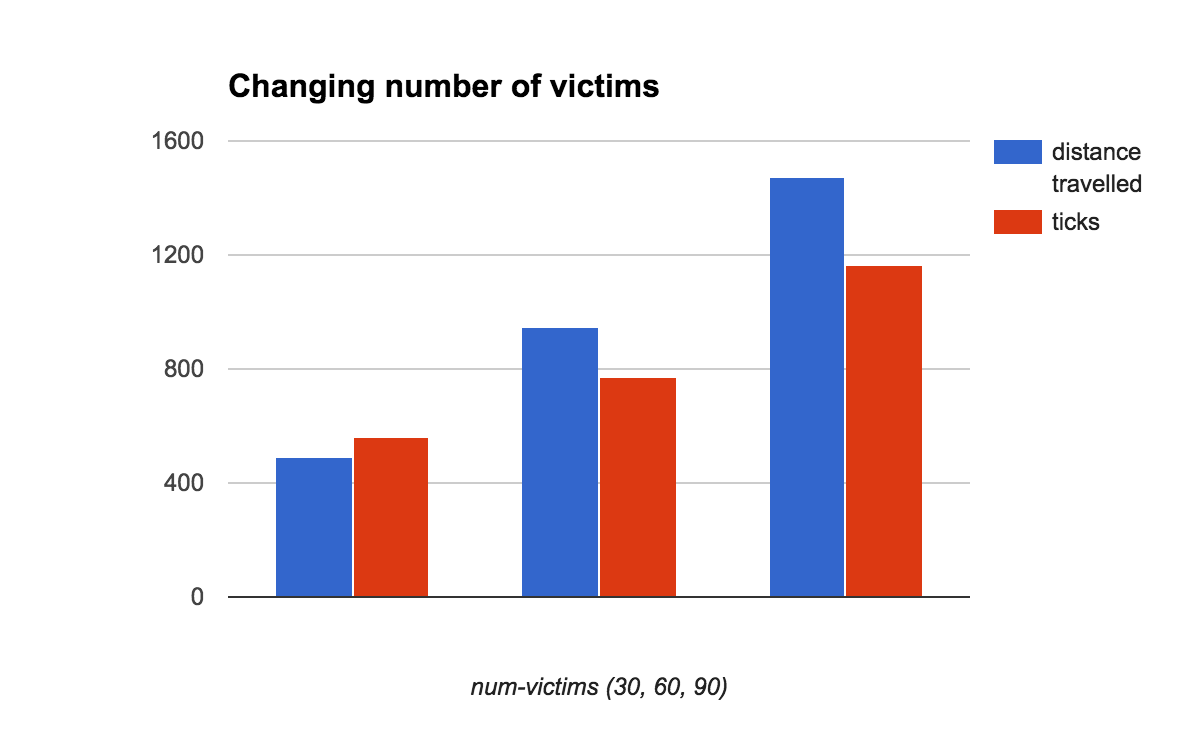
\includegraphics[width=\textwidth,height=\textheight,keepaspectratio]{2victims.png}
    \\
    The same thing is happening as in problem one, just the times are a less.
    \\
    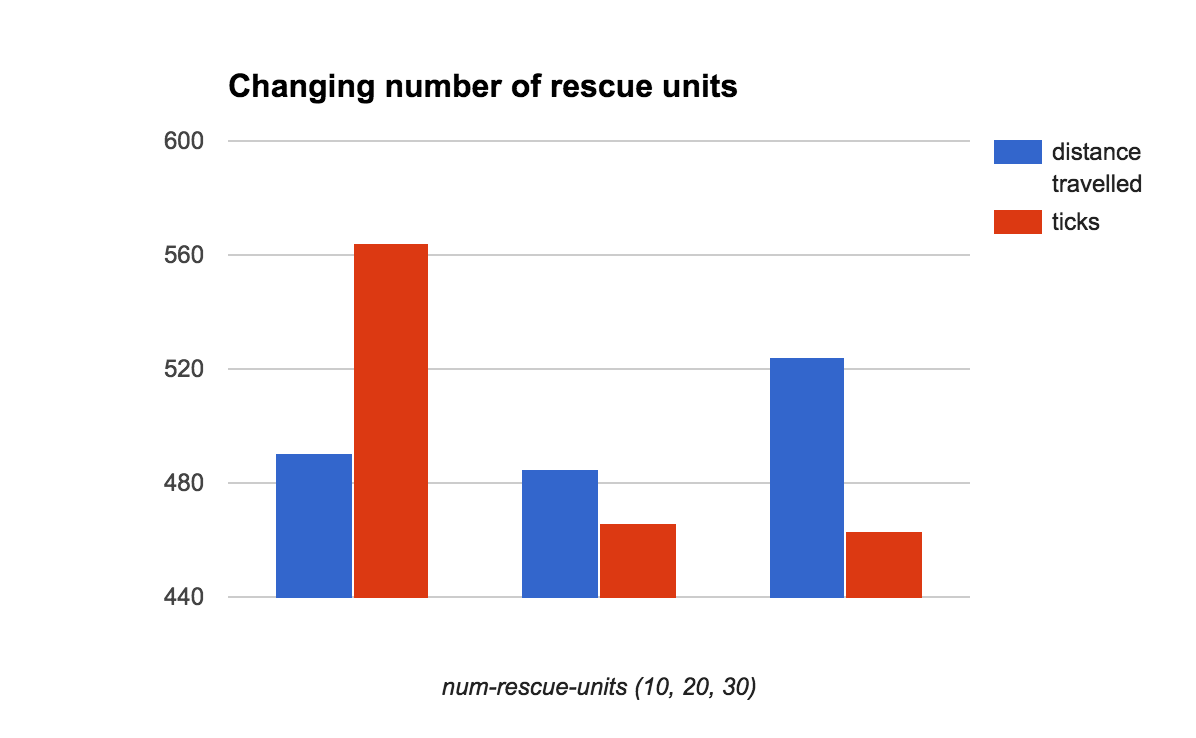
\includegraphics[width=\textwidth,height=\textheight,keepaspectratio]{2rescueunits.png}
    \\
    In the above example you can see that increasing the amount of rescue units drastically increases the time taken, This is because the ambulances are actually being smart about where they go to pick up civilians and where not to go.
    \\
    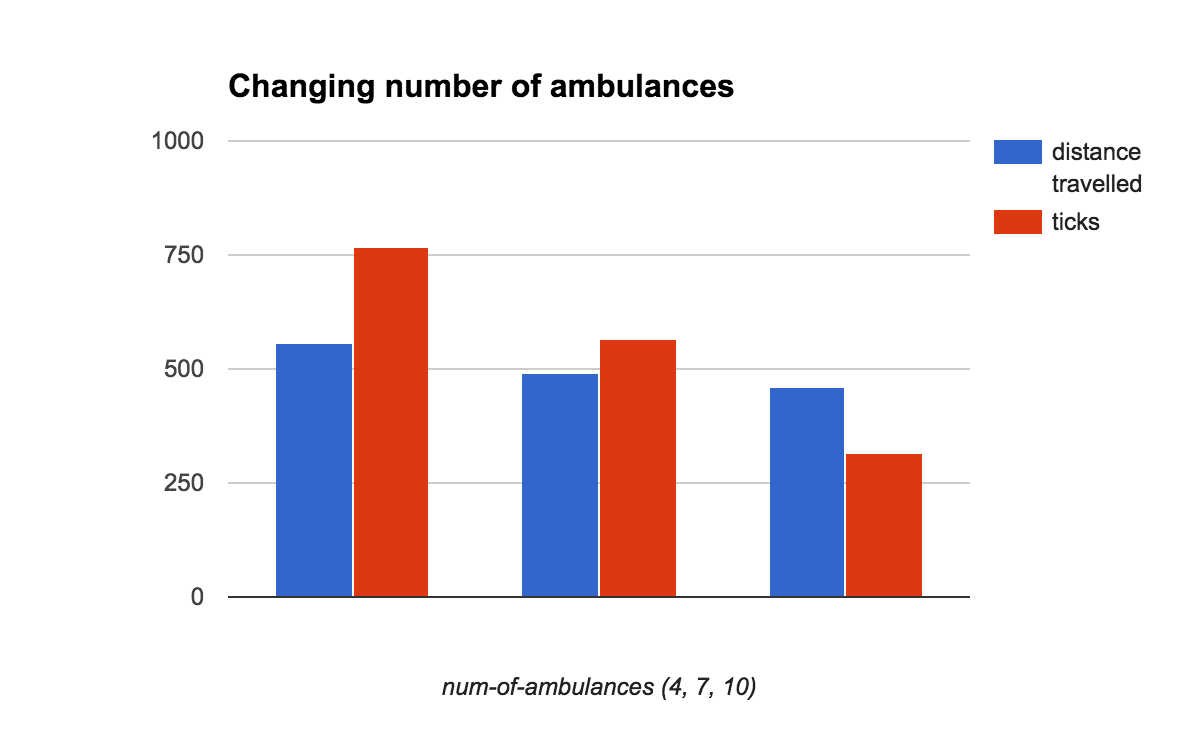
\includegraphics[width=\textwidth,height=\textheight,keepaspectratio]{2ambs.png}
    \\
    Increasing the amount of ambulances also steadily decreases the amount of time and fuel taken. This is because there is a bigger spread of ambulances to civilians.
    \\
    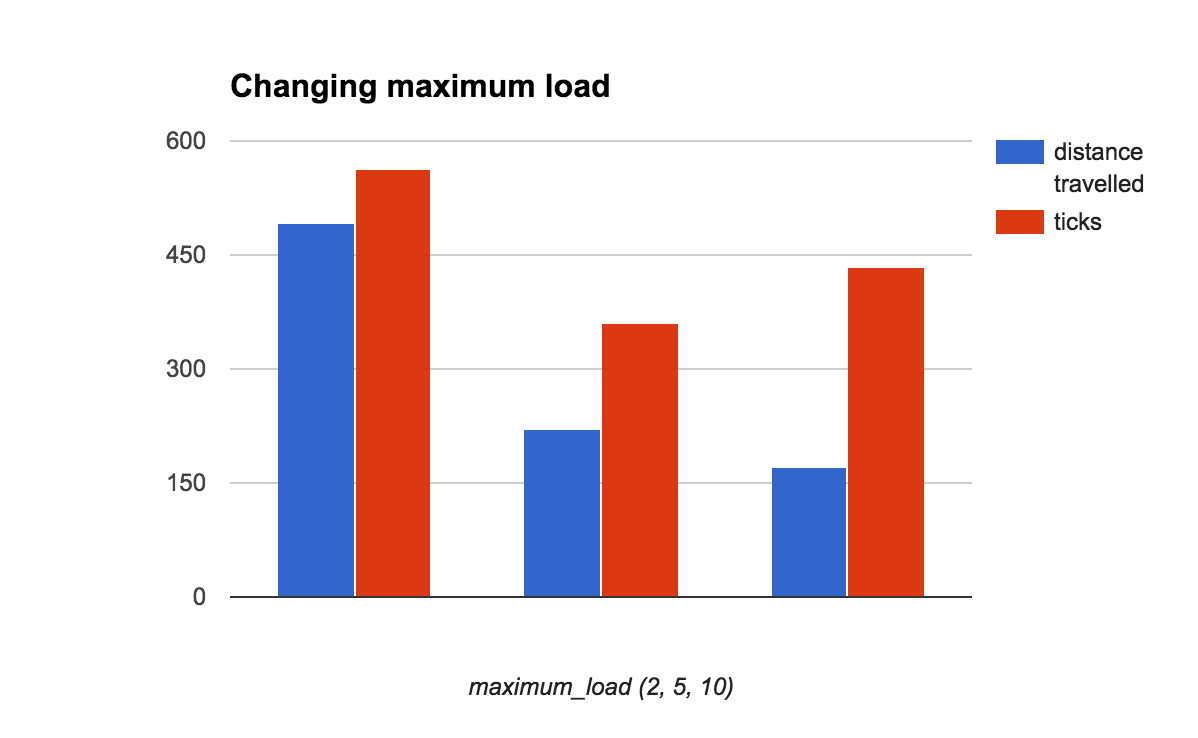
\includegraphics[width=\textwidth,height=\textheight,keepaspectratio]{2load.png}
    \\
    Although changing the maximum load decreases the distance traveled and time taken, it does hit a point where time taken increases again. I believe this is more because an ambulance my accidentally find a civilian on its way somewhere.

\section{Comparison}
  Below you can see graphs of the results side by side. In all of these graphs you can clearly see that Problem 3 is much more efficient than problem 2.

  % \\
  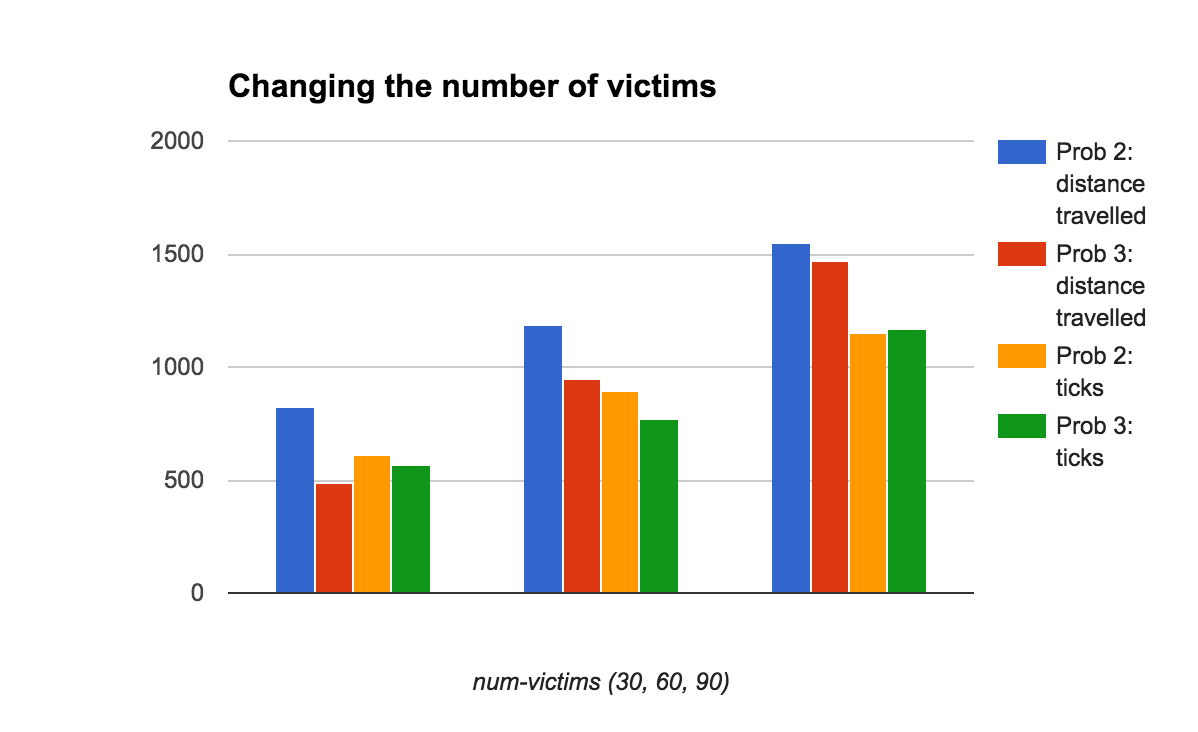
\includegraphics[width=\textwidth,height=\textheight,keepaspectratio]{3victims.png}
  % \\
  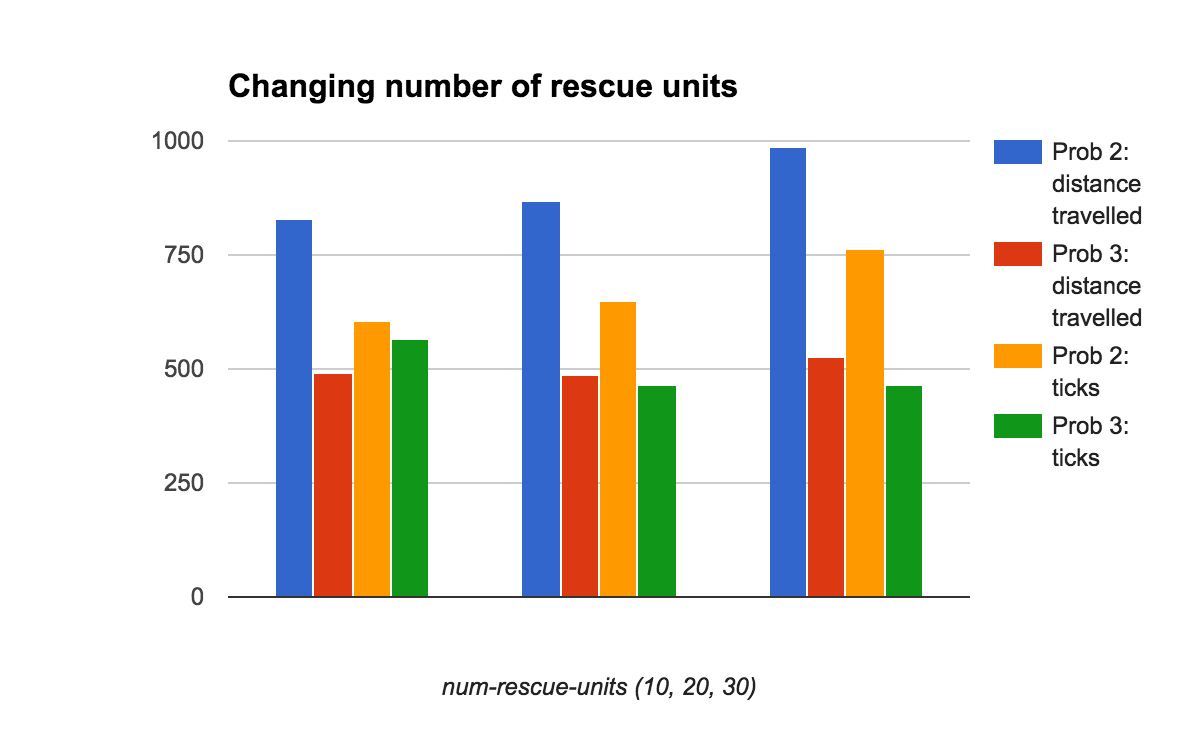
\includegraphics[width=\textwidth,height=\textheight,keepaspectratio]{3rescueunits.png}
  % \\
  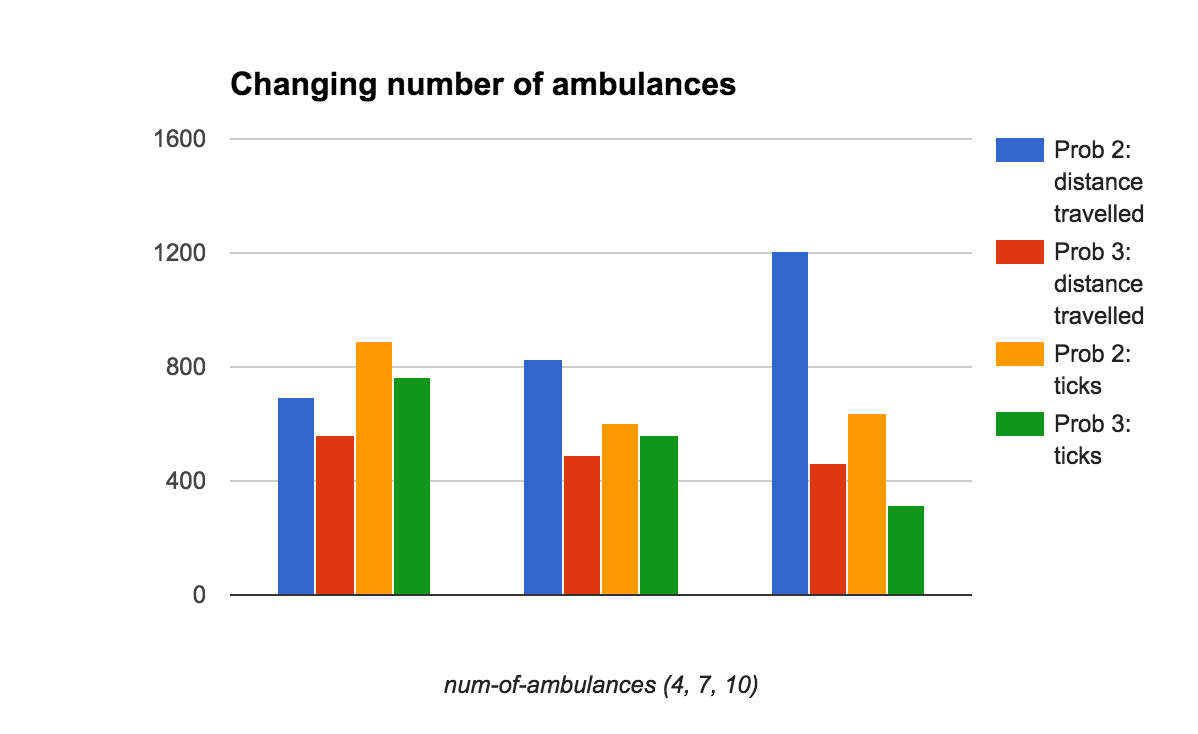
\includegraphics[width=\textwidth,height=\textheight,keepaspectratio]{3ambs.png}
  % \\
  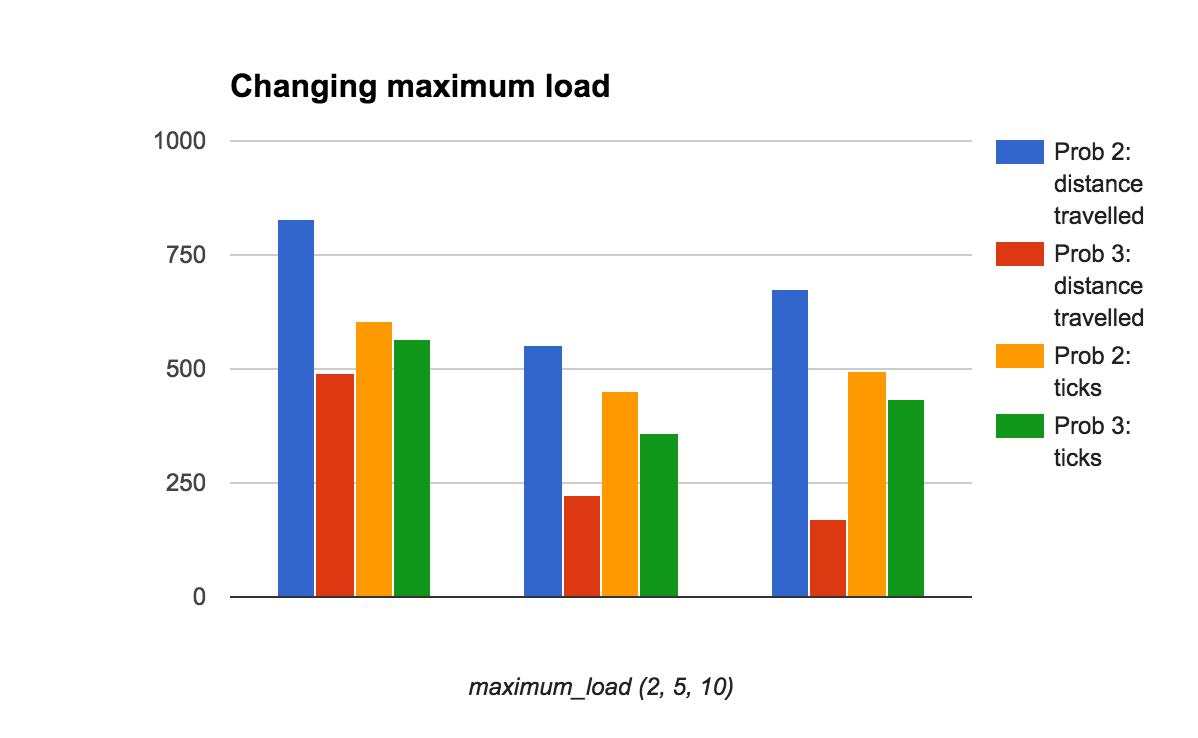
\includegraphics[width=\textwidth,height=\textheight,keepaspectratio]{3load.png}
  % \\

\end{document}